%Paulin VIOLETTE
%Si t'as pas bossé sur l'interface utilisateur t'y touche pas.
%Sauf si la personne dont le nom est écris en haut te dis d'y toucher.
%Deso Paulin moi j'y ai touché
%Putin tu casses le couilles
\chapter{Interface Utilisateur}

\section{Présentation}

%Mettre l'image de ma super interface grave stylé
\begin{figure}[h]
  \centering
  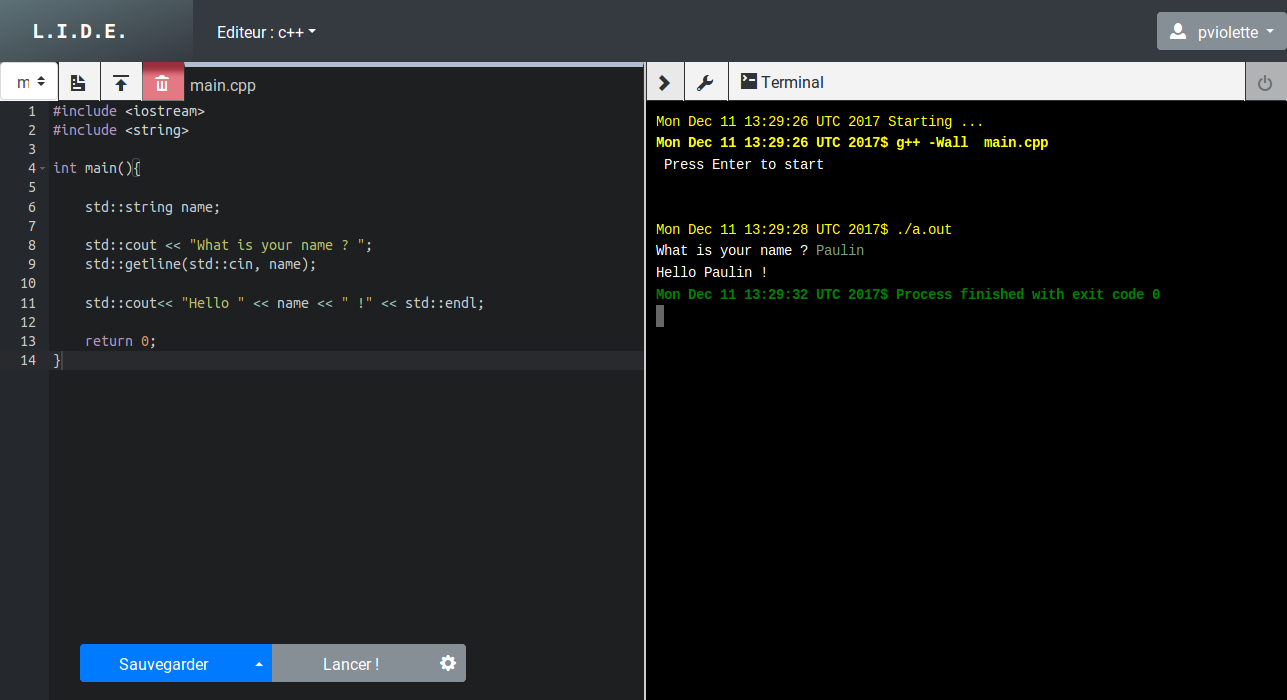
\includegraphics[width=0.8\textwidth]{./img/frontend/example1.png}
  \caption{Interface utilisateur en utilisation}
  \label{}
\end{figure}

Une fois l'utilisateur connecté, il est redirigé vers l'interface de l'application : un éditeur de texte et une console.
L'interface est divisée en quatre parties :
\begin{itemize}
  \item La barre de navigation, contenant les liens vers les autres parties du site (gestion de compte...), ainsi qu'un menu dropdown permettant de changer de langage
  \item La barre d'outils, qui contient des contrôles spécifiques à l'application (création ou importation de fichiers, contrôle de la console).
  \item L'éditeur, implémenté par le plugin Ace
  \item La console, implémentée par le plugin jqconsole
\end{itemize}

\section{Outils utilisés}
En plus des outils déjà décrits dans la section \ref{sec-principaux-outils}, l'interface utilisateur utilise plusieurs plugins Javascript.

L'éditeur de texte est Ace\footnote{Voir \url{https://ace.c9.io/}}, un éditeur de texte pour le web supportant la coloration syntaxique de près de 110 langages, mis à disposition sous licence BSD et maintenu comme le principal éditeur pour l'IDE AWS Cloud9. Cet éditeur a pour avantage de supporter de nombreuses fonctionnalités, parmi lesquelles :

\begin{itemize}
  \item L'indentation automatique
  \item Chercher/Remplacer avec des expressions régulières
  \item Changement entre tabulation avec des espaces ("soft tab") ou avec une réelle tabulation (caractère \\t, "hard tab").
  \item Numérotage des lignes
  \item Et bien d'autres...
\end{itemize}

Toutes ces raisons nous ont poussé à utiliser ce plugin.

Afin de gérer la console, nous avons choisi d'utiliser le plugin jqconsole (Plus de détails en \ref{subsec-terminal}).

Les icônes proviennent de la bibliothèque d'icônes openiconic\footnote{\url{https://useiconic.com/open}}.

Dernièrement, pour afficher les alertes relatives à l'interface, nous utilisons le plugin SweetAlert2\footnote{Voir \url{https://limonte.github.io/sweetalert2/}} qui nous permet d'avoir des alertes bien plus esthétiques que les alertes standards, et une personnalisation du contenu (champs, texte des boutons, etc...).

\section{Organisation des templates TWIG}

Le template twig de l'application, \texttt{index.html.twig}, hérite du template \texttt{layout.html.twig}, qui définit une base pour l'application, et qui contient la barre de navigation. Nous avons également créer différents templates pour les modales d'options (personnalisation, lancement, importation et création de fichier).

Les templates du bundle FOS (gérant la partie utilisateur du site) sont également redéfinis pour s'intégrer avec le reste de l'application.

\section{Environnement de Développement}

\subsection{Gestion des langages}

Une des contraintes données pour le projet était d'avoir un éditeur disposant d'une coloration syntaxique, et pouvant supporter plusieurs langages. Il nous était aussi demandé de pouvoir compiler (si besoin) et exécuter le code écrit dans ces langages. Il a donc fallu penser l'interface pour répondre à cette problématique.

Une liste des langages configurés est stockée dans la base de données, comme vu dans le chapitre \ref{ch-bdd-admin}. La page est donc génerée à partir de ces informations : un menu déroulant est inséré dans la barre de navigation, avec un choix pour chacun des langages marqués comme actifs. Le langage sélectionné est marqué via la classe CSS \texttt{.choix-langage-selected}, qui cache le lien dans le menu déroulant. Lors du chargement de la page, ou à la sélection d'un autre langage, une requête AJAX est envoyée afin de récupérer les informations sur le langage sélectionné :
\begin{itemize}
  \item le mode de l'éditeur (on appelle ensuite la méthode \texttt{setMode(mode)} sur l'éditeur Ace
  \item la liste des modèles configurés pour le langage (avec l'extension et le contenu du modèle)
  \item le nom du compilateur (utilisé dans le formulaire d'exécution pour afficher la commande de compilation qui va être exécutée)
  \item le nom du langage
\end{itemize}
Chaque lien dans le menu déroulant contient un attribut \texttt{data-id} qui permet d'identifier la langage (correspond à l'id du langage dans la base de données).

Ces informations sont ensuite utilisées pour mettre à jour l'éditeur.

\subsection{Personnalisation}

\par Toute personne ayant déjà travaillé en groupe sur un projet informatique a pu remarquer que chacun à ses préférences de thème pour un éditeur : certains préfèrent un fond sombre, d'autres un fond clair, etc... L'éditeur Ace est facilement personnalisable et dispose par défaut de 24 thèmes. Il était donc assez rapide d'implémenter un formulaire permettant à l'utilisateur de choisir le thème qui lui convient le mieux, lui permettant ainsi de facilement s'approprier son outil de travail. La police est également personnalisable.

La console ayant un style implémenté par CSS, il fut de même aisé de créer des thèmes qui s'appliquent grâce à une classe attribuée à l'élément div contenant la console. Pour l'instant, seuls trois styles de console sont implémentés, mais il serait aisé d'en ajouter d'autres dans des versions futures. Chaque style a une classe maîtresse \emph{.console-nom\_style}. On redéfinit ensuite les classes \emph{jqconsole} grâce aux sélecteurs CSS (voir le fichier \emph{console.css}).

Tous ces changements sont pour l'instant uniquement gérés en local (voir fichier \emph{options.js}).

\begin{figure}[!h]
\centering
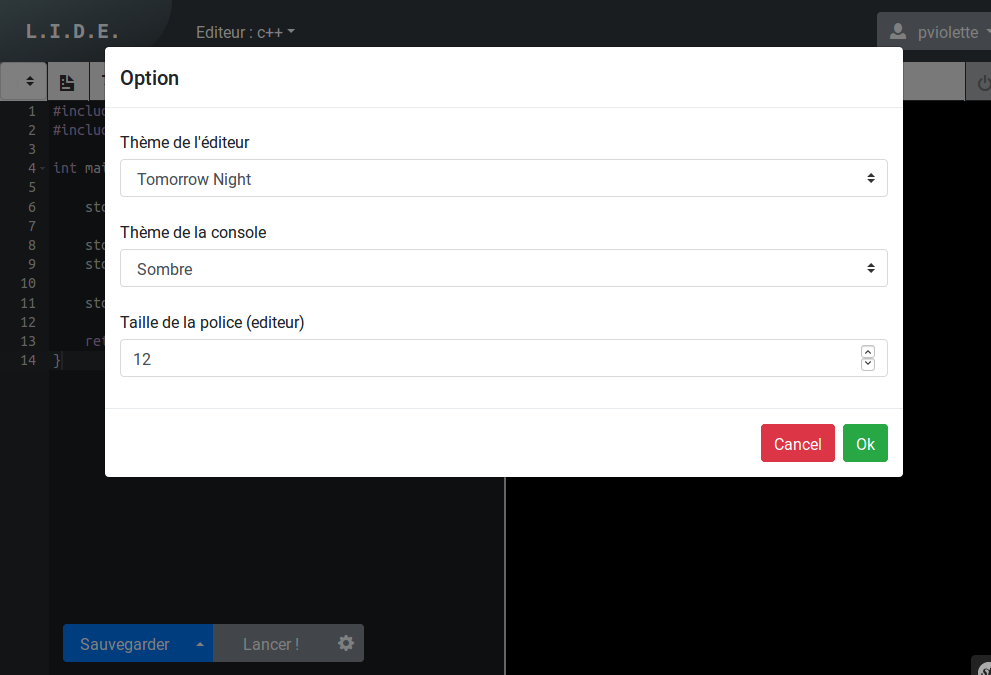
\includegraphics[width=0.8\textwidth]{./img/frontend/example_personnalisation.png}
\caption{Formulaire permettant la personnalisation de l'interface}
\end{figure}

\subsection{Gestions des fichiers}
Tel un véritable EDI, notre application permet la gestion de multiples fichiers. Cette gestion est effectuée sur le navigateur par du javascript.

Les fichiers sont enregistrés dans un prototype contenant deux champs : \emph{name}, le nom du fichier, et \emph{content} son contenu. Ces prototypes sont ensuite stockés dans la variable globale \emph{files}, un tableau de fichier. À chaque changement de fichier en cours d'édition, le contenu de l'éditeur est sauvegardé et est ensuite remplacé par le contenu du nouveau fichier à éditer.

Les fichiers peuvent être créer de deux façons : soit en important un fichier depuis son ordinateur (bouton importation), soit par création à partir de modèles définis par l'administrateur pour le langage.
On laisse également la possibilité de créer des fichiers vides (par exemple pour créer un fichier de données utilisé lors de l'exécution du programme).


\section{Compilation et exécution}

\subsection{Formulaire}

Le formulaire pour compiler et exécuter est généré par Symfony à partir de l'entity \texttt{Execution} et de la classe \texttt{ExecutionType}. Le formulaire comporte 7 champs :
\begin{itemize}
  \item Les paramètres de compilation : arguments passés au compilateur
  \item Les paramètres de lancement : arguments donnés au programme
  \item Fichiers additionnels : l'utilisateur peut choisir des fichiers depuis son ordinateur qui seront joints aux fichiers présents dans l'EDI
  \item Une option Compilation Uniquement : si activée, seule la compilation sera effectuée; le programme ne sera pas lancé
  \item{ Un choix de gestion du flux d'entrée :
  \begin{itemize}
    \item Aucun : aucune gestion des entrées n'est effectuée
    \item Interactive : entrée interactive, l'utilisateur écrit sur le flux d'entrée pendant l'exécution du programme
    \item Texte : les entrées sont définies à l'avance, le programme utilise un fichier comme flux d'entrée
  \end{itemize}}
  \item Les entrées à donner au programme : seulement si le mode de gestion des entrées Texte est sélectionné
  \item Un champs caché alimenté par le Javascript, contenant le JSON correspondant à la liste des fichiers
\end{itemize}

\subsection{Lancement de la compilation et de l'exécution}

Le lancement de la compilation et de l'exécution du code écrit est lancé par l'appui sur le bouton "Lancer" qui appelle une fonction JS envoyant une requête AJAX vers la méthode \texttt{ConsoleController::execAction} (fichier ConsoleController.php). Cette requête contient le formulaire qui est ensuite traité : les fichiers vont être écrits dans le système du fichier dans un dossier temporaire, le script de lancement et d'exécution correspondant au langage est récupéré dans la base de données et placé dans ce même répertoire. Une commande, qui va permettre de lancer le docker, est ensuite construite. Cette commande va :
\begin{itemize}
  \item Stopper le container de l'utilisateur s'il existe
  \item{Lancer un container basé sur l'image correspondante au langage, de nom \emph{id\_[id\_user]A}, paramétré pour être supprimé à la fin de l'exécution de la commande de lancement. Cette commande de lancement va :
  \begin{itemize}
    \item Récupérer le script de lancement sur le serveur de l'application via un wget
    \item Attribuer les droits d'exécution sur ce script
    \item Une commande sed remplaçant les caractères indésirables (dus à la base de données).
    \item Lancer le script avec les bons paramètres
  \end{itemize}}
\end{itemize}

Les paramètres du script à lancer sont :
\begin{itemize}
  \item \texttt{-o 'options\_de\_compilation'}, pour les paramètres à passer au compilateur
  \item \texttt{-f 'fichier1 fichier2...'}, la liste des fichiers de l'utilisateur (récupérée par un wget)
  \item \texttt{-i fichier}, le nom du fichier contenant les inputs s'il est nécessaire
  \item \texttt{-n}, pour un mode non interactif.
  \item \texttt{-a 'agr0 arg1 ...'}, les arguments à donner au programme
  \item \texttt{-c}, pour uniquement effectuer la compilation
  \item \texttt{-w 'wget\_adr'} l'adresse où effectuer le wget.
\end{itemize}

\subsection{Terminal}
\label{subsec-terminal}

\par La mise en place de la console proposait deux options : soit la création d'une vue ad-hoc soit l'intégration d'une vue déjà existante.

\par Notre choix s'est vite tourné vers l'intégration d'une vue déjà existante. La création d'une vue nous aurait certes donné une modularité de la console en ce qui concerne les modifications mais, la console une fois implémentée n'a pas nécessairement besoin de modifications.

\par Après étude de rentabilité, nous avons décidé d'implémenter la vue JQConsole \footnote{https://github.com/replit/jq-console} (utilisée dans repl.it\footnote{\url{https://repl.it/}}, un projet similaire au nôtre) qui correspondait exactement à nos besoins. En plus d'être esthétique, son code source était placé sous licence libre et toutes les fonctions qui nous étaient nécessaires étaient déjà implémentées. L'inconvénient principal est que la modification du code source peut se montrer compliquée, celui-ci étant rédigé en CoffeeScript et étant assez compliqué.

\par Nous n'avions donc plus qu'à intégrer la vue JQConsole à notre interface et faire appel aux bonnes fonctions (notamment JQConsole.Write qui permet d'afficher du texte dans la console et JQConsole.Prompt qui permet de lire du texte) pour obtenir notre console.

\section{Problèmes rencontrés et améliorations possibles}

\subsection{Rendre l'interface Responsive}
\par Un des problèmes de l'interface actuelle est son manque d'adaptabilité sur les plus petits écrans, le design actuel n'ayant pas été conçu dans le but de répondre à cette problématique. Cela est principalement dû au manque d'expérience en web qui nous a mené vers quelque chose de fonctionnel sur ordinateur qui n'est l'est pas sur les plateformes mobiles aux écrans plus petits. C'est une amélioration qu'il serait souhaitable de réaliser dans un version future.

\subsection{Persistance des options de personnalisation et de compilation}

\par Actuellement, la persistance des options de compilation ou de personnalisation n'est pas assurée. Cette fonctionnalité n'a pas été implémentée principalement par manque de temps mais pourrait rapidement être implémentée en ajoutant les champs nécessaires dans la base de données, afin de lier les préférences à un utilisateur, et en implémentant une méthode renvoyant les choix effectués dans le formulaire de personnalisation au serveur via une requête AJAX, afin que ces choix soit sauvegardés en base de données.

\subsection{Revoir la gestions des fichiers : sauvegarde de sessions plutot que simplement du contenu}
\par Actuellement, lors d'un changement de fichier, seul le contenu du fichier est sauvegardé : l'état de la session (position du curseur...) n'est pas sauvegardé. Il pourrait être intéressant de s'assurer du retour à un fichier précédemment ouvert, on retrouve exactement les mêmes conditions que dans la dernière session. Cette fonctionnalité peut être implémentée grâce aux fonctionnalités de sessions du plugin Ace, dont nous n'avons pris connaissance que trop tard.